\mfpicnumber{1}
\opengraphsfile{RationalIneq}

\setcounter{footnote}{0}

\label{RationalIneq}

In this section, we solve equations and inequalities involving rational functions and explore associated application problems. Our first example showcases the critical difference in procedure between solving a rational equation and a rational inequality.

\begin{ex}  $~$

\begin{multicols}{2}
\begin{enumerate}

\item  Solve $\dfrac{x^3-2x+1}{x-1} = \dfrac{1}{2}x-1$.

\item  Solve $\dfrac{x^3-2x+1}{x-1} \geq \dfrac{1}{2}x-1$.

\setcounter{HW}{\value{enumi}}
\end{enumerate}
\end{multicols}

\begin{enumerate}
\setcounter{enumi}{\value{HW}}

\item  Use your calculator to graphically check your answers to 1 and 2.

\end{enumerate}

{ \bf Solution.} 

\begin{enumerate}

\item  To solve the equation, we clear denominators

\[ \begin{array}{rclr}

\dfrac{x^3-2x+1}{x-1} & = & \dfrac{1}{2}x-1 & \\ [10pt]

\left(\dfrac{x^3-2x+1}{x-1}\right) \cdot 2(x-1) & = & \left( \dfrac{1}{2}x-1 \right) \cdot 2(x-1) & \\ [10pt]

2x^3 - 4x + 2 & = & x^2-3x+2 & \mbox{expand} \\

2x^3 -x^2 - x & = & 0 & \\

x(2x+1)(x-1) & = & 0 & \mbox{factor}\\

x & = & -\frac{1}{2}, \, 0, \, 1 & \\


\end{array}\]

Since we cleared denominators, we need to check for extraneous solutions.  Sure enough, we see that $x=1$ does not satisfy the original equation and must be discarded.  Our solutions are $x=-\frac{1}{2}$ and $x=0$.

\item  To solve the inequality, it may be tempting to begin as we did with the equation $-$ namely by multiplying both sides by the quantity $(x-1)$.  The problem is that, depending on $x$, $(x-1)$ may be positive (which doesn't affect the inequality) or $(x-1)$ could be negative (which would reverse the inequality).  Instead of working by cases, we collect all of the terms on one side of the inequality with $0$ on the other and make a sign diagram using the technique given on page \pageref{rationalsigndiagram} in Section \ref{RationalGraphs}.

\[ \begin{array}{rclr}

\dfrac{x^3-2x+1}{x-1} & \geq & \dfrac{1}{2}x-1 & \\ [10pt]

\dfrac{x^3-2x+1}{x-1}  - \dfrac{1}{2} x + 1& \geq & 0& \\ [10pt]

\dfrac{2\left(x^3-2x+1\right)-x(x-1)+1(2(x-1))}{2(x-1)} & \geq & 0 & \mbox{get a common denominator} \\ [10pt]

\dfrac{2x^3-x^2-x}{2x-2} & \geq & 0 & \mbox{expand} \\

\end{array} \]

Viewing the left hand side as a rational function $r(x)$ we make a sign diagram.  The only value excluded from the domain of $r$ is $x=1$ which is the solution to $2x-2=0$.  The zeros of $r$ are the solutions to $2x^3-x^2-x=0$, which we have already found to be $x=0$, $x=-\frac{1}{2}$ and $x=1$, the latter was discounted as a zero because it is not in the domain.  Choosing test values in each test interval, we construct the sign diagram below. 

\begin{center}

\begin{mfpic}[10]{-6}{6}{-2}{2}
\arrow \reverse \arrow \polyline{(-6,0),(6,0)}
\xmarks{-3,0,3}
\tlpointsep{6pt}
\axislabels {x}{{$-\frac{1}{2} \hspace{7pt}$ } -3, {$0$} 0, {$1$} 3 }
\tlabel[cc](-4.5,1){$(+)$}
\tlabel[cc](-3,1){$0$}
\tlabel[cc](-1.5,1){$(-)$}
\tlabel[cc](0,1){$0$}
\tlabel[cc](1.5,1){$(+)$}
\tlabel[cc](3,1){\textinterrobang}
\tlabel[cc](4.5,1){$(+)$}
\end{mfpic} 

\end{center}

We are interested in where $r(x) \geq 0$.  We find $r(x) > 0$, or $(+)$, on the intervals $\left(-\infty, -\frac{1}{2}\right)$, $(0,1)$ and $(1, \infty)$.  We add to these intervals the zeros of $r$, $-\frac{1}{2}$ and $0$, to get our final solution:  $\left( - \infty, -\frac{1}{2} \right] \cup [0,1) \cup (1, \infty)$.

\item  Geometrically, if we set $f(x) = \frac{x^3-2x+1}{x-1}$ and $g(x) = \frac{1}{2} x -1$, the solutions to $f(x)=g(x)$ are the $x$-coordinates of the points where the graphs of $y=f(x)$ and $y=g(x)$ intersect.  The solution to $f(x) \geq g(x)$ represents not only where the graphs meet, but the intervals over which the graph of $y=f(x)$ is above ($>$) the graph of $g(x)$. We obtain the graphs below.  

\begin{center}

\begin{tabular}{cc}

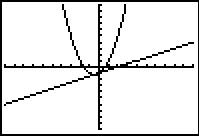
\includegraphics[width=2in]{./RationalsGraphics/Rationals10.jpg} \hspace{0.75in} & 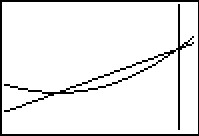
\includegraphics[width=2in]{./RationalsGraphics/Rationals11.jpg} \\


\end{tabular}
\end{center} 

The `Intersect' command confirms that the graphs cross when $x=-\frac{1}{2}$ and $x=0$.  It is clear from the calculator that the graph of $y=f(x)$ is above the graph of $y=g(x)$ on $\left(-\infty, -\frac{1}{2}\right)$ as well as on $(0,\infty)$.  According to the calculator, our solution is then $\left(-\infty, -\frac{1}{2}\right] \cup [0, \infty)$ which \textit{almost} matches the answer we found analytically.  We have to remember that $f$ is not defined at $x=1$, and, even though it isn't shown on the calculator, there is a hole\footnote{There is no asymptote at $x=1$ since the graph is well behaved near $x=1$.  According to Theorem \ref{vavshole}, there  must be a hole there.}  in the graph of $y=f(x)$ when $x=1$ which is why $x=1$ is not part of our final answer. \qed

\end{enumerate}
\end{ex}  

Next, we explore how rational equations can be used to solve some classic problems involving rates.

\begin{ex}  \label{upstreamdownstreamex}  Carl decides to explore the Meander River, the location of several recent Sasquatch sightings.  From camp, he canoes downstream five miles to check out a purported Sasquatch nest.  Finding nothing, he immediately turns around, retraces his route (this time traveling upstream), and returns to camp 3 hours after he left.  If Carl canoes at a rate  of 6 miles per hour in still water, how fast was the Meander River flowing on that day?

\smallskip

{\bf Solution.}  We are given information about distances, rates (speeds) and times.  The basic principle relating these quantities is: \[ \text{distance} = \text{rate} \cdot \text{time}\]  The first observation to make, however, is that the distance, rate and time given to us aren't `compatible':  the distance given is the distance for only \textit{part} of the trip,  the rate given is the speed Carl can canoe in still water, not in a flowing river, and  the time given is the duration of the \textit{entire} trip.  Ultimately, we are after the speed of the river, so let's call that $R$ measured in miles per hour to be consistent with the other rate given to us.  To get started, let's divide the trip into its two parts:  the initial trip downstream and the return trip upstream.  For the downstream trip, all we know is that the distance traveled is $5$ miles.

\[ \begin{array}{rcl}

\text{distance downstream} & = & \text{rate traveling downstream} \cdot \text{time traveling downstream} \\

5 \, \text{miles} & = & \text{rate traveling downstream} \cdot \text{time traveling downstream} \\ \end{array} \]

Since the return trip upstream followed the same route as the trip downstream, we know that the distance traveled upstream is also 5 miles.

\[ \begin{array}{rcl}

\text{distance upstream} & = & \text{rate traveling upstream} \cdot \text{time traveling upstream} \\

5 \, \text{miles} & = & \text{rate traveling upstream} \cdot \text{time traveling upstream} \\ \end{array} \]

We are told Carl can canoe at a  rate of $6$ miles per hour in still water.  How does this figure into the rates traveling upstream and downstream?  The speed the canoe travels in the river is a combination of the speed at which Carl can propel the canoe in still water, 6 miles per hour,  and the speed of the river, which we're calling $R$. When traveling downstream, the river is helping Carl along, so we \textit{add} these two speeds: 

\[ \begin{array}{rcl}

\text{rate traveling downstream} & = & \text{rate Carl propels the canoe} + \text{speed of the river} \\

 & = & 6 \frac{\text{miles}}{\text{hour}} + R \frac{\text{miles}}{\text{hour}} \\ \end{array} \]
 
 So our downstream speed is $(6+R) \frac{\text{miles}}{\text{hour}}$.  Substituting this into our `distance-rate-time' equation for the downstream part of the trip, we get:
 
 \[ \begin{array}{rcl}

5 \, \text{miles} & = & \text{rate traveling downstream} \cdot \text{time traveling downstream} \\ 

5 \, \text{miles} & = & (6+R) \frac{\text{miles}}{\text{hour}} \cdot \text{time traveling downstream} \\ 	\end{array} \]

 When traveling upstream, Carl works against the current.  Since the canoe manages to travel upstream,  the speed Carl can canoe in still water is greater than the river's speed, so we \textit{subtract} the river's speed \textit{from} Carl's canoing speed to get:
 
 \[ \begin{array}{rcl}

\text{rate traveling upstream} & = & \text{rate Carl propels the canoe} - \text{river speed} \\

 & = & 6 \frac{\text{miles}}{\text{hour}} - R \frac{\text{miles}}{\text{hour}} \\ \end{array} \]
 
Proceeding as before, we get
 
 \[ \begin{array}{rcl}

5 \, \text{miles} & = & \text{rate traveling upstream} \cdot \text{time traveling upstream} \\ 

5 \, \text{miles} & = & (6 - R) \frac{\text{miles}}{\text{hour}} \cdot \text{time traveling upstream} \\ 	\end{array} \]
 
The last piece of information given to us is that the total trip lasted $3$ hours.  If we let $t_{\text{down}}$ denote the time of the downstream trip and $t_{\text{up}}$ the time of the upstream trip, we have:    $t_{\text{down}} + t_{\text{up}} = 3 \, \text{hours}$.  Substituting $t_{\text{down}}$ and $t_{\text{up}}$ into the `distance-rate-time' equations, we get (suppressing the units) \textit{three} equations in \textit{three} unknowns:\footnote{This is called a \textit{system} of equations.  No doubt, you've had experience with these things before, and we will study systems in greater detail in Chapter \ref{Matrices}.} \[\left\{\begin{array}{lrcl}   E1 & (6+R) \, t_{\text{down}} & = & 5 \\ E2 & (6-R) \, t_{\text{up}} & = & 5 \\ E3 & t_{\text{down}} + t_{\text{up}} & = & 3 \end{array} \right.\]

Since we are ultimately after $R$, we need to use these three equations to get at least one equation involving only $R$.  To that end, we solve $E1$ for $t_{\text{down}}$ by dividing both sides\footnote{While we usually discourage dividing both sides of an equation by a variable expression, we know $(6+R) \neq 0$ since otherwise we couldn't possibly multiply it by $t_{\text{down}}$ and get $5$.} by the quantity $(6+R)$ to get $t_{\text{down}} = \frac{5}{6+R}$.   Similarly, we solve $E2$ for $t_{\text{up}}$ and get $t_{\text{up}} = \frac{5}{6-R}$. Substituting these into $E3$, we get:\footnote{The reader is encouraged to verify that the units in this equation are the same on both sides.  To get you started, the units on the `3' is `hours.'} \[\dfrac{5}{6+R} + \dfrac{5}{6 - R} = 3.\] Clearing denominators, we get $5(6-R) + 5(6+R) = 3(6+R)(6-R)$ which reduces to  $R^2 = 16$.   We find $R = \pm 4$, and since $R$ represents the speed of the river, we choose $R = 4$.   On the day in question, the Meander River is flowing at a rate of $4$ miles per hour. \qed

\end{ex}

One of the important lessons to learn from Example \ref{upstreamdownstreamex} is that speeds, and more generally, rates, are additive.  As we see in our next example, the concept of rate and its associated principles can be applied to a wide variety of problems - not just `distance-rate-time' scenarios.

\begin{ex} \label{workex}  Working alone, Taylor can weed the garden in 4 hours.  If Carl helps, they can weed the garden in 3 hours.  How long would it take for Carl to weed the garden on his own?

\smallskip

{\bf Solution.}  The key relationship between work and time which we use in this problem is: \[\text{amount of work done} = \text{rate of work} \cdot \text{time spent working} \]

We are told that, working alone, Taylor can weed the garden in 4 hours.  In Taylor's case then: \[ \begin{array}{rcl}

\text{amount of work Taylor does} & = & \text{rate of Taylor working} \cdot \text{time Taylor spent working} \\

1 \, \text{garden} & = & (\text{rate of Taylor working}) \cdot (4 \, \text{hours}) \\ \end{array} \]

So we have that the rate Taylor works is $\frac{1 \, \text{garden}}{ 4 \, \text{hours}} = \frac{1}{4} \frac{\text{garden}}{\text{hour}}$.    We are also told that when working together, Taylor and Carl can weed the garden in just 3 hours.  We have:

\[ \begin{array}{rcl}

\text{amount of work done together} & = & \text{rate of working together} \cdot \text{time spent working together} \\

1 \, \text{garden} & = & (\text{rate of working together}) \cdot (3 \, \text{hours}) \\ \end{array} \]

From this, we find that the rate of Taylor and Carl working together is $\frac{1 \, \text{garden}}{3 \, \text{hours}} = \frac{1}{3} \frac{\text{garden}}{\text{hour}}$.   We are asked to find out how long it would take for Carl to weed the garden on his own.  Let us call this unknown $t$, measured in hours to be consistent with the other times given to us in the problem. Then:

\[ \begin{array}{rcl}

\text{amount of work Carl does} & = & \text{rate of Carl working} \cdot \text{time Carl spent working} \\

1 \, \text{garden} & = & (\text{rate of Carl working}) \cdot (t \, \text{hours}) \\ \end{array} \]

In order to find $t$, we need to find the rate of Carl working, so let's call this quantity $R$, with units $\frac{\text{garden}}{\text{hour}}$.  Using the fact that rates are additive, we have:

\[ \begin{array}{rcl}

\text{rate working together} & = & \text{rate of Taylor working} + \text{rate of Carl working} \\ [5pt]

\frac{1}{3} \frac{\text{garden}}{\text{hour}} & = & \frac{1}{4} \frac{\text{garden}}{\text{hour}} + R \frac{\text{garden}}{\text{hour}} \\ \end{array} \]

so that $R = \frac{1}{12} \frac{\text{garden}}{\text{hour}}$.  Substituting this into our `work-rate-time' equation for Carl, we get:

\[ \begin{array}{rcl}

1 \, \text{garden} & = & (\text{rate of Carl working}) \cdot (t \, \text{hours}) \\ [5pt] 

1 \, \text{garden} & = & \left(\frac{1}{12} \frac{\text{garden}}{\text{hour}} \right) \cdot (t \, \text{hours}) \\ \end{array} \]

Solving $1 = \frac{1}{12} t$, we get $t = 12$, so it takes Carl 12 hours to weed the garden on his own.\footnote{Carl would much rather spend his time writing open-source Mathematics texts than gardening anyway.} \qed

\end{ex}

As is common with `word problems' like Examples \ref{upstreamdownstreamex} and \ref{workex}, there is no short-cut to the answer.  We encourage the reader to carefully think through and apply the basic principles of rate to each (potentially different!) situation.  It is time well spent.  We also encourage the tracking of units, especially in the early stages of the problem.  Not only does this promote uniformity in the units, it also serves as a quick means to check if an equation makes sense.\footnote{In other words, make sure you don't try to add apples to oranges!}

\smallskip

Our next example deals with the average cost function, first introduced on page \pageref{pricerevenuecostprofit}, as applied to PortaBoy Game systems from Example \ref{PortaBoyCost} in Section \ref{LinearFunctions}.

\begin{ex}  Given a cost function $C(x)$, which returns the total cost of producing $x$ items, recall that the \index{cost ! average}\index{average cost}average cost function, $\overline{C}(x) = \frac{C(x)}{x}$ computes the cost per item when $x$ items are produced.  Suppose the cost $C$, in dollars, to produce $x$ PortaBoy game systems for a local retailer is $C(x) = 80x + 150$, $x \geq 0$.

\begin{enumerate}

\item  Find an expression for the average cost function $\overline{C}(x)$. 

\item  Solve $\overline{C}(x) < 100$ and interpret.

\item  Determine the behavior of $\overline{C}(x)$ as $x \rightarrow \infty$ and interpret.


\end{enumerate}

{\bf Solution.}

\begin{enumerate}

\item  From $\overline{C}(x) = \frac{C(x)}{x}$, we obtain $\overline{C}(x) = \frac{80x+150}{x}$.  The domain of $C$ is $x \geq 0$, but since $x=0$ causes problems for $\overline{C}(x)$, we get our domain to be $x>0$, or $(0, \infty)$.

\item  Solving $\overline{C}(x) < 100$ means we solve $\frac{80x+150}{x} < 100$.  We proceed as in the previous example.

\[ \begin{array}{rclr}

\dfrac{80x+150}{x} & < & 100 & \\ [10pt]

\dfrac{80x+150}{x} - 100 & < & 0 & \\ [10pt]

\dfrac{80x + 150 - 100x}{x} & < & 0 & \mbox{common denominator} \\ [10pt]

\dfrac{150 - 20x}{x} & < & 0 & \\

\end{array} \]

If we take the left hand side to be a rational function $r(x)$, we need to keep in mind that the applied domain of the problem is $x > 0$.  This means we consider only the positive half of the number line for our sign diagram.  On $(0, \infty)$, $r$ is defined everywhere so we need only look for zeros of $r$.  Setting $r(x)=0$ gives $150-20x =0$, so that $x = \frac{15}{2}= 7.5$.  The test intervals on our domain are $(0, 7.5)$ and $(7.5, \infty)$.  We find $r(x) < 0$ on $(7.5, \infty)$.  

\begin{center}

\begin{mfpic}[10]{0}{8}{-2}{2}
\arrow \polyline{(0,0), (8,0)}
\xmarks{0,4}
\tlabel[cc](0,-1){$0$}
\tlabel[cc](0,1){\textinterrobang}
\tlabel[cc](4,-1){$7.5$}
\tlabel[cc](2,1){$(+)$}
\tlabel[cc](4,1){$0$}
\tlabel[cc](6,1){$(-)$}
\end{mfpic}

\end{center}

In the context of the problem, $x$ represents the number of PortaBoy games systems produced and $\overline{C}(x)$ is the average cost to produce each system.  Solving $\overline{C}(x) < 100$ means we are trying to find how many systems we need to produce so that the average cost is less than $\$100$ per system.  Our solution, $(7.5, \infty)$ tells us that we need to produce more than $7.5$ systems to achieve this.  Since it doesn't make sense to produce half a system, our final answer is $[8, \infty)$.

\item  When we apply Theorem \ref{hathm} to $\overline{C}(x)$ we find that $y=80$ is a horizontal asymptote to the graph of $y=\overline{C}(x)$.  To more precisely determine the behavior of $\overline{C}(x)$ as $x \rightarrow \infty$, we first use long division\footnote{In this case, long division amounts to term-by-term division.} and rewrite $\overline{C}(x) = 80+\frac{150}{x}$.  As $x \rightarrow \infty$, $\frac{150}{x} \rightarrow 0^{+}$, which means $\overline{C}(x) \approx 80 + \mbox{very small $(+)$}$.  Thus the average cost per system is getting closer to $\$ 80$ per system.  If we set $\overline{C}(x) = 80$, we get $\frac{150}{x} = 0$, which is impossible, so we conclude that $\overline{C}(x) > 80$ for all $x > 0$.  This means that the average cost per system is always greater than $\$ 80$ per system, but the average cost is approaching this amount as more and more systems are produced.  Looking back at Example \ref{PortaBoyCost}, we realize $\$ 80$ is the variable cost per system $-$ the cost per system above and beyond the fixed initial cost of $\$150$.  Another way to interpret our answer is that `infinitely' many systems would need to be produced to effectively `zero out'  the fixed cost. \qed

\end{enumerate}

\end{ex}

Our next example is another classic `box with no top' problem.

\begin{ex}  \label{boxnotopfixedvolume} A box with a square base and no top is to be constructed so that it has a volume of $1000$ cubic centimeters.  Let $x$ denote the width of the box, in centimeters as seen below.

\begin{center}

\begin{mfpic}[15]{-2}{8}{-2}{4}
\polyline{(0,0),(0,1)}
\polyline{(4,0), (4,1)}
\polyline{(0,1),(2,3)}
\polyline{(4,1),(6,3)}
\polyline{(0,0),(4,0)}
\polyline{(0,1),(4,1)}
\polyline{(2,3),(6,3)}
\polyline{(4,0),(6,2)}
\polyline{(6,3),(6,2)}
\polyline{(2,3),(2,2)}
\polyline{(2,2),(5,2)}
\dotted \polyline{(5,2),(6,2)}
\polyline{(2,2),(1,1)}
\dotted \polyline{(1,1),(0,0)}
\arrow \reverse \arrow \polyline{(0,-0.5),(4,-0.5)}
\tlabel[cc](2,-1.5){\scriptsize width, $x$}
\arrow \reverse \arrow \polyline{(-0.5,0), (-0.5,1)}
\tlabel[cc](-1.5,0.5){\scriptsize height}
\arrow \reverse \arrow \polyline{(4.5, -0.25), (6.5,1.75)}
\tlabel[cc](6,0.25){\scriptsize depth}
\end{mfpic}


\end{center}


\begin{enumerate}

\item  Express the height $h$ in centimeters as a function of the width $x$ and state the applied domain.

\item  Solve $h(x) \geq x$ and interpret.

\item  Find and interpret the behavior of $h(x)$ as $x \rightarrow 0^{+}$ and as $x \rightarrow \infty$.

\item  Express the surface area $S$ of the box as a function of $x$ and state the applied domain.

\item  Use a calculator to approximate (to two decimal places) the dimensions of the box which minimize the surface area.

\end{enumerate}

{ \bf Solution.}

\begin{enumerate}

\item  We are told that the volume of the box is $1000$ cubic centimeters and that $x$ represents the width, in centimeters.  From geometry, we know $\mbox{Volume} = \mbox{width} \times \mbox{height} \times \mbox{depth}$.  Since the base of the box is a square, the width and the depth are both $x$ centimeters.  Using $h$ for the height, we have $1000 = x^2h$, so that $h = \frac{1000}{x^2}$.  Using function notation,\footnote{That is, $h(x)$ means `$h$ of $x$', not `$h$ times $x$' here.} $h(x) = \frac{1000}{x^2}$  As for the applied domain, in order for there to be a box at all, $x > 0$, and since every such choice of $x$ will return a positive number for the height $h$ we have no other restrictions and  conclude our domain is $(0, \infty)$.

\item  To solve $h(x) \geq x$, we proceed as before and collect all nonzero terms on one side of the inequality in order to use a sign diagram.

\[ \begin{array}{rclr}

h(x) & \geq & x & \\ [10pt]

\dfrac{1000}{x^2} & \geq & x & \\ [10pt]

\dfrac{1000}{x^2} - x & \geq & 0 \\ [10pt]

\dfrac{1000-x^3}{x^2} & \geq & 0 & \mbox{common denominator} \\[10pt]

\end{array} \]

We consider the left hand side of the inequality as our rational function $r(x)$.  We see $r$ is undefined at $x=0$, but, as in the previous example, the applied domain of the problem is $x > 0$, so we are considering only the behavior of $r$ on $(0, \infty)$.  The sole zero of $r$ comes when $1000-x^3 = 0$, which is $x=10$.  Choosing test values in the intervals $(0,10)$ and $(10, \infty)$ gives the following diagram.

\begin{center}

\begin{mfpic}[10]{0}{8}{-2}{2}

\arrow \polyline{(0,0), (8,0)}

\xmarks{0,4}

\tlabel[cc](0,-1){$0$}

\tlabel[cc](0,1){\textinterrobang}

\tlabel[cc](2,1){$(+)$}

\tlabel[cc](4,-1){$10$}

\tlabel[cc](4,1){$0$}

\tlabel[cc](6,1){$(-)$}

\end{mfpic}

\end{center}

We see $r(x) > 0$ on $(0,10)$, and since $r(x) = 0$ at $x=10$, our solution is $(0,10]$.  In the context of the problem, $h$ represents the height of the box while $x$ represents the width (and depth) of the box.  Solving $h(x) \geq x$ is tantamount to finding the values of $x$ which result in a box where the height is at least as big as the width (and, in this case, depth.)  Our answer tells us the width of the box can be at most $10$ centimeters for this to happen.

\item As $x \rightarrow 0^{+}$, $h(x) = \frac{1000}{x^2} \rightarrow \infty$.  This means that the smaller the width $x$  (and, in this case, depth), the larger the height $h$ has to be in order to maintain a volume of $1000$ cubic centimeters. As $x \rightarrow \infty$, we find $h(x) \rightarrow 0^{+}$, which means that in order to maintain a volume of $1000$ cubic centimeters, the width and depth must get bigger as the height becomes smaller.

\item  Since the box has no top, the surface area can be found by adding the area of each of the sides to the area of the base.  The base is a square of dimensions $x$ by $x$, and each side has dimensions $x$ by $h$.  We get the surface area, $S = x^2+4xh$.  To get $S$ as a function of $x$, we substitute $h = \frac{1000}{x^2}$ to obtain $S = x^2+4x \left( \frac{1000}{x^2}\right)$.  Hence, as a function of $x$, $S(x) = x^2 + \frac{4000}{x}$.  The domain of $S$ is the same as $h$, namely $(0, \infty)$, for the same reasons as above.

\item   A first attempt at the graph of $y=S(x)$ on the calculator may lead to frustration.  Chances are good that the first window chosen to view the graph will suggest $y=S(x)$ has the $x$-axis as a horizontal asymptote.  From the formula $S(x) = x^2 + \frac{4000}{x}$, however, we get $S(x) \approx x^2$ as $x \rightarrow \infty$, so $S(x) \rightarrow \infty$.  Readjusting the window, we find $S$ does possess a relative minimum at $x \approx 12.60$.  As far as we can tell,\footnote{without Calculus, that is...} this is the only relative extremum, so it is the absolute minimum as well. This means that the width and depth of the box should each measure approximately $12.60$ centimeters.  To determine the height, we find $h(12.60) \approx 6.30$, so the height of the box should be approximately $6.30$ centimeters.

\begin{center}

\begin{tabular}{ccc}

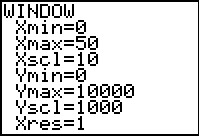
\includegraphics[width=1.75in]{./RationalsGraphics/Rationals12.jpg}  & 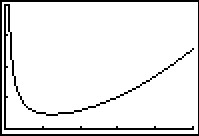
\includegraphics[width=1.75in]{./RationalsGraphics/Rationals13.jpg} & 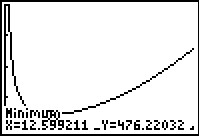
\includegraphics[width=1.75in]{./RationalsGraphics/Rationals14.jpg} \\


\end{tabular}
\end{center} 

\end{enumerate}
\qed

\end{ex}


\subsection{Variation}
\label{Variation}

In many instances in the sciences, rational functions are encountered as a result of fundamental natural laws which are typically a result of assuming certain basic relationships between variables.  These basic relationships are summarized in the definition below.

\smallskip

\colorbox{ResultColor}{\bbm

\begin{defn} \label{variation}  Suppose $x$, $y$ and $z$ are variable quantities.  We say

\begin{itemize}

\item  $y$ \index{variation ! direct}\index{direct variation}\textbf{varies directly with} (or is \textbf{directly proportional to}) $x$ if there is a constant $k$ such that $y=kx$.

\item  $y$ \index{variation ! inverse}\index{inverse variation}\textbf{varies inversely with} (or is \textbf{inversely proportional to}) $x$ if there is a constant $k$ such that $y=\frac{k}{x}$.

\item  $z$ \index{variation ! joint}\index{joint variation}\textbf{varies jointly with} (or is \textbf{jointly proportional to}) $x$ and $y$ if there is a constant $k$ such that $z = kxy$.


\end{itemize}

The constant $k$ in the above definitions is called the \index{variation ! constant of proportionality}\index{constant of proportionality}\textbf{constant of proportionality}.

\end{defn}

\ebm}

\smallskip

\begin{ex}  Translate the following into mathematical equations using Definition \ref{variation}.

\begin{enumerate}

\item  \href{http://en.wikipedia.org/wiki/Hooke's_law}{\underline{Hooke's Law}}:  \index{Hooke's Law} The force $F$ exerted on a spring is directly proportional the extension $x$ of the spring.

\item  \href{http://en.wikipedia.org/wiki/Boyle's_law}{\underline{Boyle's Law}}:  \index{Boyle's Law} At a constant temperature, the pressure $P$ of an ideal gas is inversely proportional to its volume $V$.

\item  The volume $V$ of a right circular cone varies jointly with the height $h$ of the cone and the square of the radius $r$ of the base.

\item  \href{http://en.wikipedia.org/wiki/Ohm's_law}{\underline{Ohm's Law}}:  \index{Ohm's Law} The current $I$ through a conductor between two points is directly proportional to the voltage $V$ between the two points and inversely proportional to the resistance $R$ between the two points.

\item \label{gravitylaw} \href{http://en.wikipedia.org/wiki/Law_of_universal_gravitation}{\underline{Newton's Law of Universal Gravitation}}:  \index{Newton's Law of Universal Gravitation} Suppose two objects, one of mass $m$ and one of mass $M$, are positioned so that the distance between their centers of mass is $r$.  The gravitational force $F$ exerted on the two objects varies directly with the product of the two masses and inversely with the square of the distance between their centers of mass.

\end{enumerate}

{\bf Solution.}  

\begin{enumerate}

\item Applying the definition of direct variation, we get  $F = k x$ for some constant $k$.

\item Since $P$ and $V$ are inversely proportional, we write $P = \frac{k}{V}$.

\item  There is a bit of ambiguity here.  It's clear that the volume and the height of the cone are represented by the quantities $V$ and $h$, respectively, but does $r$ represent the radius of the base or the square of the radius of the base?  It is the former.  Usually, if an algebraic operation is specified (like squaring), it is meant to be expressed in the formula.  We apply Definition \ref{variation} to get $V = k h r^{2}$.  

\item  Even though the problem doesn't use the phrase `varies jointly', it is implied by the fact that the current $I$ is related to two different quantities.  Since $I$ varies directly with $V$ but inversely with $R$, we write $I = \frac{k V}{R}$.

\item We write the product of the masses $mM$ and the square of the distance as $r^2$.  We have that $F$ varies directly with $mM$ and inversely with $r^2$, so $F = \frac{kmM}{r^2}$.  \qed

\end{enumerate}

\end{ex}

In many of the formulas in the previous example, more than two varying quantities are related.  In practice, however, usually all but two quantities are held constant in an experiment and the data collected is used to relate just two of the variables.  Comparing just two varying quantities allows us to view the relationship between them as functional, as the next example illustrates.

\begin{ex}  According to this \href{http://web.lemoyne.edu/~giunta/classicalcs/boyleverify.html}{\underline{website}} the actual data relating the volume $V$ of a gas and its pressure $P$ used by Boyle and his assistant in 1662 to verify the gas law that bears his name is given below.

\[ \begin{array}{|c||c|c|c|c|c|c|c|c|c|c|c|c|c|}  \hline

V & 48 & 46 & 44 & 42 & 40 & 38 & 36 & 34 & 32 & 30 & 28 & 26 & 24  \\ \hline

P & 29.13 & 30.56 & 31.94 & 33.5 & 35.31 & 37 & 39.31 & 41.63 & 44.19 & 47.06 & 50.31 & 54.31 & 58.81  \\ \hline \end{array} \]


\[\begin{array}{|c||c||c|c|c|c|c|c|c|c|c|c|c|c|} \hline

V & 23 & 22 & 21 & 20 & 19 & 18 & 17 & 16 & 15 & 14 & 13 & 12  \\ \hline 

P & 61.31 & 64.06 & 67.06 & 70.69 & 74.13 & 77.88 & 82.75 & 87.88 & 93.06 & 100.44 & 107.81 & 117.56   \\ \hline \end{array} \]

\begin{enumerate}

\item  Use your calculator to generate a scatter diagram for these data using $V$ as the independent variable and $P$ as the dependent variable.  Does it appear from the graph that $P$ is inversely proportional to $V$?  Explain.

\item  Assuming that $P$ and $V$ do vary inversely, use the data to approximate the constant of proportionality.

\item  Use your calculator to determine a `Power Regression' for this data\footnote{We will talk more about this in the coming chapters.} and use it verify your results in 1 and 2.


\end{enumerate}


{\bf Solution.}


\begin{enumerate}

\item If $P$ really does vary inversely with $V$, then $P = \frac{k}{V}$ for some constant $k$.  From the data plot, the points do seem to lie along a curve like $y = \frac{k}{x}$.

\item  To determine the constant of proportionality, we note that from $P = \frac{k}{V}$, we get $k = PV$.  Multiplying each of the volume numbers times each of the pressure numbers,\footnote{You can use tell the calculator to do this arithmetic on the lists and save yourself some time.} we produce a number which is always approximately $1400$.  We suspect that $P = \frac{1400}{V}$.  Graphing $y = \frac{1400}{x}$ along with the data gives us good reason to believe our hypotheses that $P$ and $V$ are, in fact, inversely related.

\begin{center}

\begin{tabular}{cc}

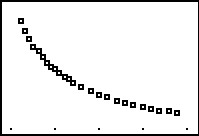
\includegraphics[width=2in]{./RationalsGraphics/Rationals15.jpg} \hspace{0.75in} & 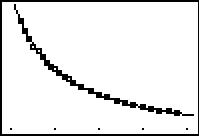
\includegraphics[width=2in]{./RationalsGraphics/Rationals16.jpg} \\

The graph of the data  \hspace{0.75in} & The data with $y=\frac{1400}{x}$ \\


\end{tabular}
\end{center} 



\item  After performing a `Power Regression', the calculator fits the data to the curve $y = ax^b$ where $a \approx 1400$ and $b \approx -1$ with a correlation coefficient which is darned near perfect.\footnote{We will revisit this example once we have developed logarithms in Chapter \ref{ExpLogs} to see how we can actually `linearize' this data and do a linear regression to obtain the same result.}  In other words, $y = 1400 x^{-1}$ or $y = \frac{1400}{x}$, as we guessed.


\begin{center}

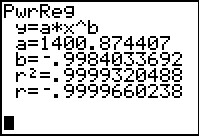
\includegraphics[width=2in]{./RationalsGraphics/Rationals17.jpg}

\end{center} 

\qed

\end{enumerate}

\end{ex}

\newpage

\subsection{Exercises}

In Exercises \ref{ratleqnexercisefirst} - \ref{ratleqnexerciselast},  solve the rational equation.  Be sure to check for extraneous solutions.

\begin{multicols}{2}
\begin{enumerate}

\item $\dfrac{x}{5x + 4} = 3$ \label{ratleqnexercisefirst}
\item $\dfrac{3x - 1}{x^{2} + 1} = 1$

\setcounter{HW}{\value{enumi}}
\end{enumerate}
\end{multicols}

\begin{multicols}{2}
\begin{enumerate}
\setcounter{enumi}{\value{HW}}

\item $\dfrac{1}{x + 3} + \dfrac{1}{x - 3} = \dfrac{x^{2} - 3}{x^{2} - 9}$
\item $\dfrac{2x + 17}{x + 1} = x + 5$

\setcounter{HW}{\value{enumi}}
\end{enumerate}
\end{multicols}

\begin{multicols}{2}
\begin{enumerate}
\setcounter{enumi}{\value{HW}}
\item $\dfrac{x^{2} - 2x + 1}{x^{3} + x^{2} - 2x} = 1$
\item $\dfrac{-x^{3} + 4x}{x^{2} - 9} = 4x$  \label{ratleqnexerciselast}

\setcounter{HW}{\value{enumi}}
\end{enumerate}
\end{multicols}

In Exercises \ref{ratlineqexercisefirst} - \ref{ratlineqexerciselast}, solve the rational inequality.  Express your answer using interval notation.

\begin{multicols}{3}
\begin{enumerate}
\setcounter{enumi}{\value{HW}}

\item $\dfrac{1}{x + 2} \geq 0$ \label{ratlineqexercisefirst}
\item $\dfrac{x - 3}{x + 2} \leq 0$
\item $\dfrac{x}{x^{2} - 1} > 0$

\setcounter{HW}{\value{enumi}}
\end{enumerate}
\end{multicols}

\begin{multicols}{3}
\begin{enumerate}
\setcounter{enumi}{\value{HW}}


\item  $\dfrac{4x}{x^2+4} \geq 0$
\item  $\dfrac{x^2-x-12}{x^2+x-6} > 0$
\item  $\dfrac{3x^2-5x-2}{x^2-9} < 0$

\setcounter{HW}{\value{enumi}}
\end{enumerate}
\end{multicols}

\begin{multicols}{3}
\begin{enumerate}
\setcounter{enumi}{\value{HW}}


\item  $\dfrac{x^3+2x^2+x}{x^2-x-2} \geq 0$
\item $\dfrac{x^{2} + 5x + 6}{x^{2} - 1} > 0$
\item $\dfrac{3x - 1}{x^{2} + 1} \leq 1$

\setcounter{HW}{\value{enumi}}
\end{enumerate}
\end{multicols}

\begin{multicols}{3}
\begin{enumerate}
\setcounter{enumi}{\value{HW}}

\item $\dfrac{2x + 17}{x + 1} > x + 5$
\item $\dfrac{-x^{3} + 4x}{x^{2} - 9} \geq 4x$
\item $\dfrac{1}{x^{2} + 1} < 0$ 

\setcounter{HW}{\value{enumi}}
\end{enumerate}
\end{multicols}

\begin{multicols}{2}
\begin{enumerate}
\setcounter{enumi}{\value{HW}}

\item $\dfrac{x^4-4x^3+x^2-2x-15}{x^3-4x^2} \geq x$
\item $\dfrac{5x^3-12x^2+9x+10}{x^2-1}\geq 3x-1$ \label{ratlineqexerciselast}

\setcounter{HW}{\value{enumi}}
\end{enumerate}
\end{multicols}

\begin{enumerate}
\setcounter{enumi}{\value{HW}}


\item  Carl and Mike start a 3 mile race at the same time.  If Mike ran the race at 6 miles per hour and finishes the race 10 minutes before Carl, how fast does Carl run?

\item  One day, Donnie observes that the wind is blowing at 6 miles per hour.  A unladen swallow nesting near Donnie's house flies three quarters of a mile down the road (in the direction of the wind), turns around, and returns exactly 4 minutes later.  What is the airspeed of the unladen swallow?  (Here, `airspeed' is the speed that the swallow can fly in still air.) 

\item  In order to remove water from a flooded basement, two pumps, each rated at 40 gallons per minute, are used. After half an hour, the one pump burns out, and the second pump finishes removing the water half an hour later.  How many gallons of water were removed from the basement?

\item  A faucet can fill a sink in 5 minutes while a drain will empty the same sink in 8 minutes.  If the faucet is turned on and the drain is left open, how long will it take to fill the sink?

\item Working together, Daniel and Donnie can clean the llama pen in 45 minutes.  On his own, Daniel can clean the pen in an hour.  How long does it take Donnie to clean the llama pen on his own?

\item  In Exercise \ref{newportaboycost}, the function $C(x) = .03x^{3} - 4.5x^{2} + 225x + 250$, for $x \geq 0$ was used to model the cost (in dollars) to produce $x$ PortaBoy game systems. Using this cost function, find the number of PortaBoys which should be produced to minimize the average cost $\overline{C}$.  Round your answer to the nearest number of systems. 

\item  Suppose we are in the same situation as Example \ref{boxnotopfixedvolume}.  If the volume of the box is to be $500$ cubic centimeters, use your calculator to find the dimensions of the box which minimize the surface area.  What is the minimum surface area?  Round your answers to two decimal places.

\item  The box for the new Sasquatch-themed cereal, `Crypt-Os', is to have a volume of $140$ cubic inches.  For aesthetic reasons, the height of the box needs to be $1.62$ times the width of the base of the box.\footnote{1.62 is a crude approximation of the so-called `Golden Ratio' $\phi = \frac{1 + \sqrt{5}}{2}$.}  Find the dimensions of the box which will minimize the surface area of the box.  What is the minimum surface area?  Round your answers to two decimal places.   

\item \label{fixedareaminperimetergarden} Sally is Skippy's neighbor from Exercise \ref{fixedperimetermaxareagarden} in Section \ref{QuadraticFunctions}.   Sally also wants to plant a vegetable garden along the side of her home.  She doesn't have any fencing, but wants to keep the size of the garden to 100 square feet.  What are the dimensions of the garden which will minimize the amount of fencing she needs to buy?  What is the minimum amount of fencing she needs to buy? Round your answers to the nearest foot. (Note:  Since one side of the garden will border the house, Sally doesn't need fencing along that side.)



\item Another Classic Problem: A can is made in the shape of a right circular cylinder and is to hold one pint. (For dry goods, one pint is equal to $33.6$ cubic inches.)\footnote{According to \href{http://dictionary.reference.com/browse/pint}{\underline{www.dictionary.com}}, there are different values given for this conversion.  We will stick with $33.6 \mbox{in}^{3}$ for this problem.}  

\begin{enumerate}

\item Find an expression for the volume $V$ of the can in terms of the height $h$ and the base radius $r$.
\item Find an expression for the surface area $S$ of the can in terms of the height $h$ and the base radius $r$.  (Hint: The top and bottom of the can are circles of radius $r$ and the side of the can is really just a rectangle that has been bent into a cylinder.)
\item Using the fact that $V = 33.6$, write $S$ as a function of $r$ and state its applied domain.
\item Use your graphing calculator to find the dimensions of the can which has minimal surface area.

\end{enumerate}

\item  A right cylindrical drum is to hold 7.35 cubic feet of liquid.  Find the dimensions (radius of the base and height) of the drum which would minimize the surface area.  What is the minimum surface area?  Round your answers to two decimal places.


\item In Exercise \ref{Sasquatchfunc1} in Section \ref{FunctionNotation}, the population of Sasquatch in Portage County was modeled by the function $P(t) = \frac{150t}{t + 15}$, where $t = 0$ represents the year 1803.  When were there fewer than 100 Sasquatch in Portage County?

\setcounter{HW}{\value{enumi}}
\end{enumerate}


In Exercises \ref{varexercisefirst} - \ref{varexerciselast},  translate the following into mathematical equations.

\begin{enumerate}
\setcounter{enumi}{\value{HW}}

\item  At a constant pressure, the temperature $T$ of an ideal gas is directly proportional to its volume $V$.  (This is \href{http://en.wikipedia.org/wiki/Charles's_law}{\underline{Charles's Law}}) \index{Charles's Law} \label{varexercisefirst}

\item  The frequency of a wave $f$ is inversely proportional to the wavelength of the wave $\lambda$.

\item  The density $d$ of a material is directly proportional to the mass of the object $m$ and inversely proportional to its volume $V$.

\item  The square of the orbital period of a planet $P$ is directly proportional to the cube of the semi-major axis of its orbit $a$. (This is \href{http://en.wikipedia.org/wiki/Kepler}{\underline{Kepler's Third Law of Planetary Motion }}) \index{Kepler's Third Law of Planetary Motion}

\item  The drag of an object traveling through a fluid $D$ varies jointly with the density of the fluid $\rho$ and the square of the velocity of the object $\nu$.

\item Suppose two electric point charges, one with charge $q$ and one with charge $Q$, are positioned $r$ units apart. The electrostatic force $F$ exerted on the charges varies directly with the product of the two charges and inversely with the square of the distance between the charges. (This is \href{http://en.wikipedia.org/wiki/Electrostatic#Coulomb.27s_law}{\underline{Coulomb's Law}}) \index{Coulomb's Law} \label{varexerciselast}

\setcounter{HW}{\value{enumi}}
\end{enumerate}

\begin{enumerate}
\setcounter{enumi}{\value{HW}}

\item According to \href{http://en.wikipedia.org/wiki/Vibrating_string}{\underline{this webpage}}, the frequency $f$ of a vibrating string is given by $f = \dfrac{1}{2L} \sqrt{\dfrac{T}{\mu}}$ where $T$ is the tension, $\mu$ is the linear mass\footnote{Also known as the linear density.  It is simply a measure of mass per unit length.} of the string and $L$ is the length of the vibrating part of the string.  Express this relationship using the language of variation.

\item According to the Centers for Disease Control and Prevention \href{http://www.cdc.gov}{\underline{www.cdc.gov}}, a person's Body Mass Index $B$ is directly proportional to his weight $W$ in pounds and inversely proportional to the square of his height $h$ in inches. \index{BMI, body mass index}

\begin{enumerate}

\item Express this relationship as a mathematical equation. \label{BMIfirst} 
\item If a person who was $5$ feet, $10$ inches tall weighed 235 pounds had a Body Mass Index of 33.7, what is the value of the constant of proportionality? \label{BMIsecond}
\item Rewrite the mathematical equation found in part \ref{BMIfirst} to include the value of the constant found in part \ref{BMIsecond} and then find your Body Mass Index.

\end{enumerate}

\item We know that the circumference of a circle varies directly with its radius with $2\pi$ as the constant of proportionality. (That is, we know $C = 2\pi r.$)  With the help of your classmates, compile a list of other basic geometric relationships which can be seen as variations.

\end{enumerate}

\newpage

\subsection{Answers}

\begin{multicols}{3} 
\begin{enumerate}

\item $x = -\frac{6}{7}$
\item $x = 1, \; x = 2$
\item $x = -1$

\setcounter{HW}{\value{enumi}}
\end{enumerate}
\end{multicols}

\begin{multicols}{3}
\begin{enumerate}
\setcounter{enumi}{\value{HW}}

\item $x = -6, \; x = 2$
\item No solution
\item $x = 0, \; x = \pm 2\sqrt{2}$

\setcounter{HW}{\value{enumi}}
\end{enumerate}
\end{multicols}

\begin{multicols}{2}
\begin{enumerate}
\setcounter{enumi}{\value{HW}}

\item $(-2, \infty)$
\item $(-2, 3]$

\setcounter{HW}{\value{enumi}}
\end{enumerate}
\end{multicols}

\begin{multicols}{2}
\begin{enumerate}
\setcounter{enumi}{\value{HW}}


\item $(-1, 0) \cup (1, \infty)$
\item $[0, \infty)$

\setcounter{HW}{\value{enumi}}
\end{enumerate}
\end{multicols}

\begin{multicols}{2}
\begin{enumerate}
\setcounter{enumi}{\value{HW}}

\item $(-\infty, -3) \cup (-3,2) \cup (4, \infty)$
\item $\left(-3, -\frac{1}{3} \right) \cup (2,3)$

\setcounter{HW}{\value{enumi}}
\end{enumerate}
\end{multicols}

\begin{multicols}{2}
\begin{enumerate}
\setcounter{enumi}{\value{HW}}

\item $(-1,0] \cup (2, \infty)$
\item $(-\infty, -3) \cup (-2, -1) \cup (1, \infty)$

\setcounter{HW}{\value{enumi}}
\end{enumerate}
\end{multicols}

\begin{multicols}{2}
\begin{enumerate}
\setcounter{enumi}{\value{HW}}

\item $(-\infty, 1] \cup [2, \infty)$
\item $(-\infty, -6) \cup (-1, 2)$

\setcounter{HW}{\value{enumi}}
\end{enumerate}
\end{multicols}

\begin{multicols}{2}
\begin{enumerate}
\setcounter{enumi}{\value{HW}}

\item $(-\infty, -3) \cup \left[-2\sqrt{2}, 0\right] \cup \left[2\sqrt{2}, 3\right)$
\item No solution

\setcounter{HW}{\value{enumi}}
\end{enumerate}
\end{multicols}

\begin{multicols}{2}
\begin{enumerate}
\setcounter{enumi}{\value{HW}}

\item $[-3,0) \cup (0,4) \cup [5, \infty)$
\item  $\left(-1,-\frac{1}{2}\right] \cup (1, \infty)$

\setcounter{HW}{\value{enumi}}
\end{enumerate}
\end{multicols}


\begin{multicols}{3}
\begin{enumerate}
\setcounter{enumi}{\value{HW}}

\item  4.5 miles per hour

\item  24 miles per hour

\item  3600 gallons

\setcounter{HW}{\value{enumi}}
\end{enumerate}
\end{multicols}

\begin{multicols}{3}
\begin{enumerate}
\setcounter{enumi}{\value{HW}}

\item  $\frac{40}{3} \approx 13.33$ minutes

\item 3 hours

\setcounter{HW}{\value{enumi}}
\end{enumerate}
\end{multicols}

\begin{enumerate}
\setcounter{enumi}{\value{HW}}

\item  The absolute minimum of $y=\overline{C}(x)$ occurs at $\approx (75.73, 59.57)$.  Since $x$ represents the number of game systems, we check $\overline{C}(75) \approx 59.58$ and $\overline{C}(76) \approx 59.57$.  Hence, to minimize the average cost, $76$ systems should be produced at an average cost of $\$59.57$ per system.

\item The width (and depth) should be $10.00$ centimeters, the height should be $5.00$ centimeters.  The minimum surface area is $300.00$ square centimeters.

\item The width of the base of the box should be $\approx 4.12$ inches, the height of the box should be $\approx 6.67$ inches, and the depth of the base of the box should be $\approx 5.09$ inches;  minimum surface area $\approx 164.91$ square inches.

\item The dimensions are  $\approx 7$ feet by $\approx 14$ feet;  minimum amount of fencing required $\approx 28$ feet.

\item 

\begin{multicols}{2}
\begin{enumerate}

\item $V = \pi r^{2}h$
\item $S = 2 \pi r^{2} + 2\pi r h$

\setcounter{HWindent}{\value{enumii}}
\end{enumerate}
\end{multicols}

\begin{multicols}{2}
\begin{enumerate}
\setcounter{enumii}{\value{HWindent}}

\item $S(r) = 2\pi r^{2} + \frac{67.2}{r}, \;$  Domain $r > 0$
\item $r \approx 1.749\,$in. and $h \approx 3.498\,$in. 

\end{enumerate}
\end{multicols}

\item  The radius of the drum should be $\approx 1.05$ feet and the height of the drum should be $\approx 2.12$ feet.  The minimum surface area of the drum is $\approx 20.93$ cubic feet.

\item $P(t) < 100$ on $(-15, 30)$, and the portion of this which lies in the applied domain is $[0,30)$.  Since $t=0$ corresponds to the year 1803, from 1803 through the end of 1832, there were fewer than 100 Sasquatch in Portage County.

\setcounter{HW}{\value{enumi}}
\end{enumerate}

\begin{multicols}{3}
\begin{enumerate}
\setcounter{enumi}{\value{HW}}

\item $T = k V$

\item \hspace{-.1in} \footnote{The character $\lambda$ is the lower case Greek letter `lambda.'} $f = \dfrac{k}{\lambda}$

\item $d = \dfrac{k m}{V}$ 

\setcounter{HW}{\value{enumi}}
\end{enumerate}
\end{multicols}


\begin{multicols}{3}
\begin{enumerate}
\setcounter{enumi}{\value{HW}}

\item $P^2 = k a^3$

\item \hspace{-.1in} \footnote{The characters $\rho$ and $\nu$ are the lower case Greek letters `rho' and `nu,' respectively.} $D = k \rho \nu^2$

\item \hspace{-.1in} \footnote{Note the similarity to this formula and Newton's Law of Universal Gravitation as discussed in Example \ref{gravitylaw}.}  $F = \dfrac{kqQ}{r^2}$   

\setcounter{HW}{\value{enumi}}
\end{enumerate}
\end{multicols}

\begin{enumerate}
\setcounter{enumi}{\value{HW}}

\item Rewriting $f = \dfrac{1}{2L} \sqrt{\dfrac{T}{\mu}}$ as $f = \dfrac{\frac{1}{2} \sqrt{T}}{L \sqrt{\mu}}$ we see that the frequency $f$ varies directly with the square root of the tension and varies inversely with the length and the square root of the linear mass.

\item \begin{multicols}{3} 
\begin{enumerate}
\item $B = \dfrac{kW}{h^{2}}$
\item \hspace{-.1in} \footnote{The CDC uses 703.} $k = 702.68$ 
\item $B = \dfrac{702.68W}{h^{2}}$
\end{enumerate}
\end{multicols}


\end{enumerate}


\closegraphsfile